% begin module continuity-ex2
\begin{frame}
\begin{example}[Example 2a, p. 114]
Where is this function discontinuous?
\begin{columns}[c]
\column{.4\textwidth}
\[
f(x) = \frac{x^2 - x - 2}{\alert<handout:0 |3>{x - 2}}
\]
\ \uncover<4->{
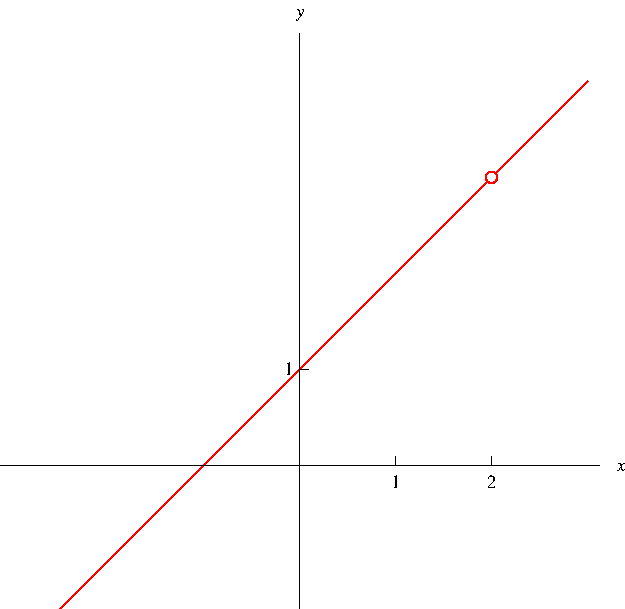
\includegraphics[height=4.5cm]{continuity/pictures/02-05-ex2a.pdf}%
}
\column{.6\textwidth}
\begin{itemize}
\item<2-| alert@2-3>  $f(2)$ \uncover<3->{doesn't exist.}
\item<4->  Discontinuous at 2.
\item<5->  This is called a removable discontinuity because we could remove it by redefining $f$ at the single number 2.
\end{itemize}
\end{columns}
\end{example}
\end{frame}



\begin{frame}
\begin{example}[Example 2b, p. 114]
Where is this function discontinuous?
\begin{columns}[c]
\column{.4\textwidth}
\[
f(x) = \left\{ \begin{array}{lcl}
\frac{1}{\alert<handout:0 |6>{x^2}} & \text{ if } & x \neq 0 \\
\alert<handout:0 |4>{1} & \alert<handout:0 |4>{\text{ if }} & \alert<handout:0 |4>{x = 0} \\
\end{array}\right.
\]
\ 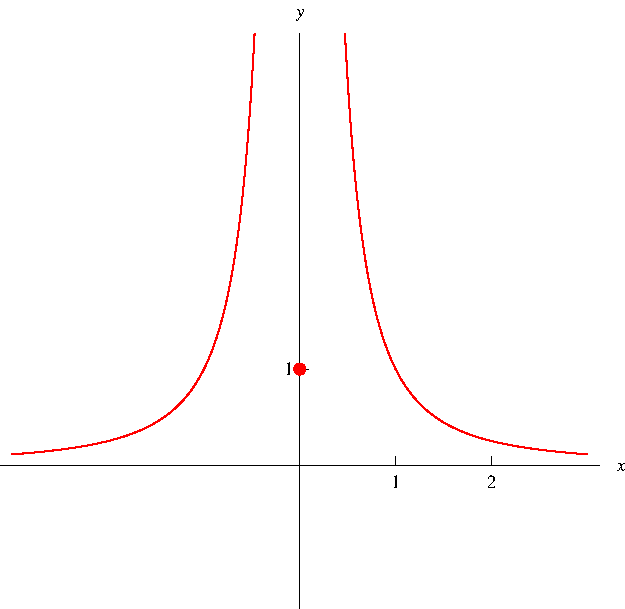
\includegraphics[height=4.5cm]{continuity/pictures/02-05-ex2b.pdf}%
\column{.6\textwidth}
\begin{itemize}
\item<2-| alert@3-4>  $f(0)$ \uncover<4->{exists ($f(0) = 1$).}
\item<2-| alert@5-6>  $\lim_{x\rightarrow 0} f(x)$ \uncover<6->{doesn't exist ($\infty$).}
\item<7->  Discontinuous at 0.
\item<8->  This is called an infinite discontinuity. 
\end{itemize}
\end{columns}
\end{example}
\end{frame}


\begin{frame}
\begin{example}[Example 2c, p. 114]
Where is this function discontinuous?
\begin{columns}[c]
\column{.4\textwidth}
\[
f(x) = \left\{ \begin{array}{lcl}
\frac{x^2 - x - 2}{x-2} & \text{ if } & x \neq 2 \\
\alert<handout:0 |4>{1} & \alert<handout:0 |4>{\text{ if }} & \alert<handout:0 |4>{x = 2} \\
\end{array}\right.
\]
\ 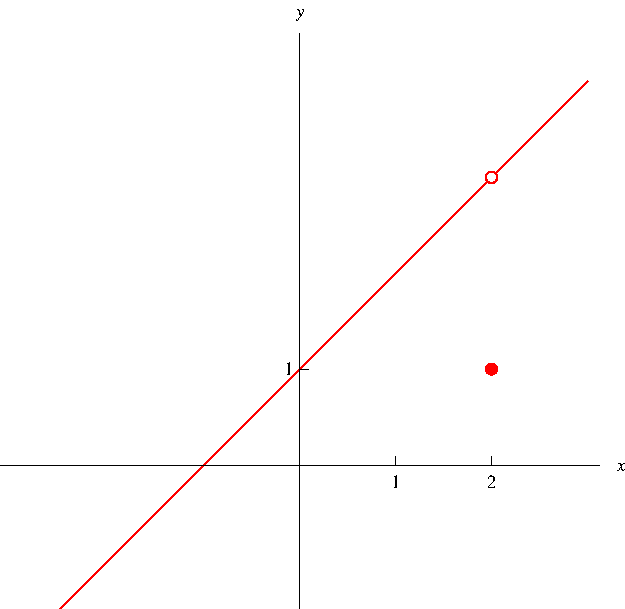
\includegraphics[height=4.5cm]{continuity/pictures/02-05-ex2c.pdf}%
\column{.6\textwidth}
\begin{itemize}
\item<2-| alert@3-4>  $f(2)$ \uncover<4->{exists ($f(2) = 1$).}
\item<2-| alert@5-6>  $\lim_{x\rightarrow 2} f(x)$ \uncover<6->{exists ($3$).}
\item<7->  $\lim_{x\rightarrow 2}f(x) \neq f(2)$.
\item<8->  Discontinuous at 2.
\item<9->  This is also a removable discontinuity.
\end{itemize}
\end{columns}
\end{example}
\end{frame}



\begin{frame}
\begin{example}[Example 2d, p. 114]
Where is this function discontinuous?
\begin{columns}[c]
\column{.4\textwidth}
\[
f(x) = [[x]]
\]
\ 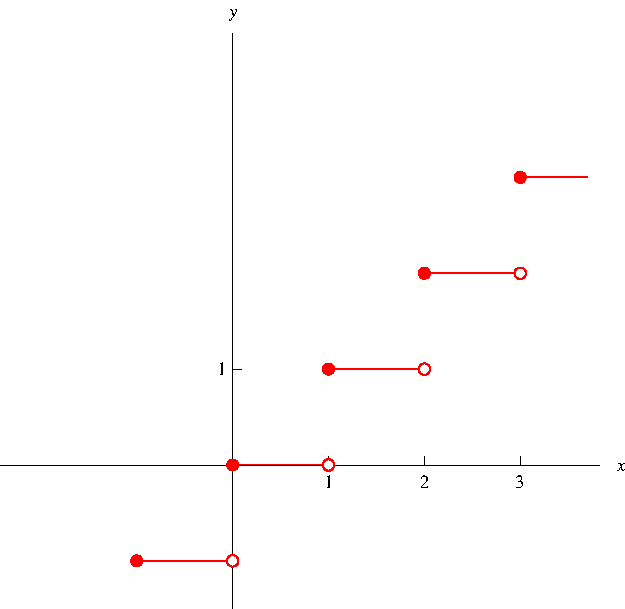
\includegraphics[height=4.5cm]{continuity/pictures/02-05-ex2d.pdf}%
\column{.6\textwidth}
\begin{itemize}
\item<2-| alert@3-4>  $f(1)$ \uncover<4->{exists ($f(1) = 1$).}
\item<2-| alert@5-6>  $\lim_{x\rightarrow 1^+} f(x)$ \uncover<6->{$ = 1$.}
\item<2-| alert@7-8>  $\lim_{x\rightarrow 1^-} f(x)$ \uncover<8->{$ = 0$.}
\item<2-| alert@9-10>  $\lim_{x\rightarrow 1} f(x)$ \uncover<10->{doesn't exist.}
\item<11->  Discontinuous at 1.
\item<12->  Discontinuous at every integer $n$.
\item<13->  These are called jump discontinuities because the function ``jumps'' at these numbers (i.e., the left limit doesn't equal the right limit).
\end{itemize}
\end{columns}
\end{example}
\end{frame}
% end module continuity-ex2
